\documentclass[runningheads,a4paper]{llncs}

\usepackage{amssymb}
\setcounter{tocdepth}{3}
\usepackage{graphicx}

\usepackage[utf8]{inputenc}
\usepackage[unicode=true,hidelinks]{hyperref}

\usepackage{url}
\newcommand{\keywords}[1]{\par\addvspace\baselineskip
\noindent\keywordname\enspace\ignorespaces#1}

\usepackage{hyperref}
\usepackage{listings}
%\usepackage[scaled]{luximono}


%\usepackage{natbib}

% ----- begin macros

\lstdefinelanguage{Scala}%
{morekeywords={abstract,%
  case,catch,char,class,%
  def,else,extends,final,for,%
  if,import,implicit,%
  match,module,%
  new,null,%
  object,override,%
  package,private,protected,public,%
  for,public,return,super,%
  this,throw,trait,try,type,%
  val,var,%
  with,%
  yield,%
  lazy%
  },%
  sensitive,%
  morecomment=[l]//,%
  morecomment=[s]{/*}{*/},%
  morestring=[b]",%
  morestring=[b]',%
  showstringspaces=false%
}[keywords,comments,strings]%

\lstdefinelanguage{JavaScript}%
{morekeywords={for, var, attributes, class, classend, do, else, empty, endif, endwhile, fail, function,
functionend, if, implements, in, inherit, inout, not, of, operations, out, return,
then, types, while, use},%
  sensitive,%
  morecomment=[l]//,%
  morecomment=[s]{/*}{*/},%
  morestring=[b]",%
  morestring=[b]',%
  showstringspaces=false%
}[keywords,comments,strings]%

\lstset{language=Scala,%
  mathescape=false,%
%  columns=[c]fixed,%
  aboveskip=\smallskipamount,
  belowskip=\smallskipamount,
%  basewidth={0.5em, 0.4em},%
  basicstyle=\ttfamily\small,%
  keywordstyle=\bfseries%\sffamily\bfseries,%
%  keywordstyle=\sffamily\bfseries,%
%  xleftmargin=0.5cm
}

\newcommand{\commentstyle}[1]{\slseries{#1}}
\newcommand{\keywordstyle}[1]{\bfseries{#1}}

\lstnewenvironment{slisting}{\lstset{language=Scala}}{}

\newcommand{\code}[1]{\lstinline[language=Scala,columns=fixed,basicstyle=\ttfamily\small]|#1|}

\def\changemargin#1#2{\list{}{\rightmargin#2\leftmargin#1}\item[]}
\let\endchangemargin=\endlist

%\setlength{\columnseprule}{0.25pt}

%\renewcommand{\note}[1]{$\spadesuit$ \textbf{#1} $\clubsuit$}


%\newcommand{\comment}[1]{}


\newcommand{\ie}{\emph{i.e.}}
\newcommand{\eg}{\emph{e.g.}}
\newcommand{\cf}{\emph{cf.~}}
\newcommand{\etal}{\emph{et al.~}}
\newcommand{\etc}{\emph{etc.}}
\newcommand{\aka}{\emph{a.k.a.}}


\begin{document}

\mainmatter

\title{Using Path-Dependent Types to Build Safe JavaScript Foreign Function Interfaces}
%\titlerunning{Dependent Types Rock}

\author{Julien Richard-Foy \and Olivier Barais\and Jean-Marc Jézéquel}
\authorrunning{Julien Richard-Foy \emph{et. al.}}

\institute{IRISA, Université de Rennes 1, France. \texttt{\{first\}.\{last\}@irisa.fr}}

%\toctitle{Lecture Notes in Computer Science}
%\tocauthor{Authors' Instructions}
\maketitle


\begin{abstract}
Several programming languages can target JavaScript as a back-end, giving developers programming
language features that are absent from JavaScript, such as static typing. However, the Web browser
APIs, which are needed to interact with a Web page, are designed for JavaScript, making it
challenging to expose them in a statically typed language. Indeed, existing statically typed
languages exposing Web browser APIs either break type safety or give developers less control than if
they were using JavaScript. This article shows how to expose Web browser APIs in Scala in a type
safe way while keeping the same level of control as with native APIs by using path-dependent types
and functional dependencies. We validate this approach in designing safe and concise foreign
function interfaces between Scala and JavaScript for DOM events handling and DOM manipulation. We
compared this approach to common frameworks such as GWT, Fay, Kotlin, Dart and SharpKit.
\keywords{Path-Dependent Types, JavaScript, Scala, Foreign Function Interface}
\end{abstract}


\section{Introduction}

Web applications are attractive because they require no installation or deployment step on clients
and enable large scale collaborative experiences. Besides, now they can be executed
efficiently~\cite{Gal:2009:TJT:1542476.1542528} on top of modern web-browsers. However, writing
large Web applications is known to be
difficult~\cite{Mikkonen08_SpaghettiJs,Preciado05_RIAMethodologyNecessity}. One challenge comes from
the fact that the JavaScript programming language -- which is currently the only action language
natively supported by almost all Web clients -- lacks of constructs making large code bases
maintainable (\eg static typing, first-class modules).

One solution consists in considering JavaScript as an assembly language\footnote{\cf
\href{http://asmjs.org/}{http://asmjs.org/}} and generating JavaScript from compilers of
full-featured and cutting-edge programming languages. Incidentally, an increasing number of
programming languages or compiler back-ends can generate JavaScript code (\eg
Java/GWT~\cite{Chaganti07_GWT},
SharpKit\footnote{\href{http://sharpkit.net}{http://sharpkit.net}}, Dart~\cite{Griffith11_Dart},
Kotlin\footnote{\href{http://kotlin.jetbrains.org/}{http://kotlin.jetbrains.org/}},
ClojureScript~\cite{McGranaghan11_ClojureScript},
Fay\footnote{\href{http://fay-lang.org/}{http://fay-lang.org/}}, Haxe~\cite{Cannasse08_HaXe},
Opa\footnote{\href{http://opalang.org/}{http://opalang.org/}}). However, compiling to JavaScript is
not enough. Developers also need the Web browser programming environment: they need to interact with
the Web page, to build DOM fragments, to listen to user events, \etc. A Foreign Function
Interface (FFI) mechanism could be used to make browser’s APIs available to the developers. However,
JavaScript APIs are not statically typed and make a heavy use of overloading, making them hard to
expose in a statically typed language.

Indeed, existing statically typed languages compiling to JavaScript often expose weaker types than
they should. For instance, the function \code{createElement} is polymorphic in its return type: it
can return a \code{DivElement} as well as an \code{InputElement}, among others, but the Dart, Fay,
SharpKit and Kotlin APIs return the super-type of all the possible values, namely the \code{Element}
type. As a consequence, developers need to explicitly down-cast the value they get, which is a
tedious and error prone task.

Some other languages try to workaround this problem by using overloading instead of polymorphism.
For instance, HaXe provides functions \code{createDivElement}, \code{createInputElement}, which
return a \code{DivElement} and an \code{InputElement}, respectively. Besides requiring a higher
effort to implement, this solution also reduces the control level of users: by being statically
resolved, the element type can not anymore be passed as a parameter.

It turns out that most of the existing statically typed languages compiling to JavaScript either
loose control or loose type safety when they expose Web browser’s APIs. How to give developers the
same level of control as if they were using the native Web APIs, but in a statically typed and
convenient way?

In this paper we present several ways to integrate Web browser’s APIs as statically typed APIs that
are safe and give developers the same control level as if they were using the native APIs. We
achieve this by using advanced features of type systems like dependent types and functional
dependencies. We validate this approach in designing safe FFI between Scala and JavaScript for DOM
events handling and DOM manipulation. We compared this approach to common frameworks such as GWT,
Fay, Kotlin, Dart and SharpKit.


The outline of this paper is the following.
Section~\ref{sec:background} presents several motivating example and gives a background about
path-dependent type.
Section~\ref{sec:jsscala} presents %...
Section~\ref{sec:evaluation} validates our ideas through the design of FFI for DOM events handling
and DOM manipulation in Scala and compare these FFIs w.r.t. the existing FFIs for these features
within frameworks such as GWT, Fay, Kotlin, Dart and SharpKit.
Section~\ref{sec:related} discusses related work, Section~\ref{sec:conclusion} concludes this paper
and highlights  future work. 


\section{Background Material}

\subsection{Foreign Function Interface}

A FFI is a mechanism that allows a programmer to link one programming language program to programs
written in another language. Such mechanisms exist in lots of languages: Ada, Java, Haskell, Lisp or
GWT. Despite the name, FFIs are not necessarily restricted to function calls; many FFIs permit
method calls on objects; and some even permit migration of non-trivial datatypes and/or objects
across the language boundary. Nevertheless, the challenging tasks come when you want to: (i) manage
shared garbage collection policies, (ii) handle the conversion of complex datatype to map from one
environment to another and (iii) handle the design of safe foreign function interfaces regarding
typing system constraints that can differ from one environment to another. This last issue is the
one which is targeted in this paper for the design of FFI between a statically typed language such
as Scala and a dynamically typed language such as JavaScript.


\subsection{Path-Dependent Type Overview}

A type system provides us a near mathematical proof that programs that compile successfully obey a
set of rules and restrictions and, as such, are bug-free in that respect. For example, after
compiling a Java program, developer knows that it will not do a division of a number with a
string and that, if our method foo receives an integer as argument, it will not be called anywhere
with an argument of any type other than an integer. Among all the type theory,  dependent types is a term that describes using values as types, the type depends on a value. This means you can encode some properties of an object in its type. Once you do
that, it allows a type checker (a compiler) to verify that the object (type) is used in a suitable
way. Scala has the concept of abstract types: types
that, just like abstract methods, must be defined by subclasses. Objects can have a type as members. On top of this abstract type, Scala defines a concept of path-dependent type.  As the term path-dependent type says, the type depends on the path: in general, different paths give
rise to different types. In the example of Figure~\ref{pathdependenttypeexample}\footnote{highly inspired from https://github.com/milessabin/shapeless\#sized-types}, we show how the size of the list can be used as a type information. We define a function row that convert a list of element into a printed html array, we define a function html that takes a list of size N as a first parameter and a list of list of size N as a second parameter. We use the path dependent type to create these type lists: \emph{Sized}. Consequently if we use this function \emph{html} with a list of three elements (\textit{headers}) and a list of list of 3 elements (\textit{rows}), the program compiles and runs correctly. If we use  this function \emph{html} with a list of four elements (\textit{extendedHeaders}) and a list of list of 3 elements (\textit{rows}), it does not compiled. 



\begin{figure}
\begin{lstlisting}[label=pathdependenttypeexample,caption=Path dependent type example]
//functions definition
def row(cols : Seq[String]) 
	= cols.mkString("<td>", "</td> <td>", "</td>")
def html[N <: Nat]
	(hdrs : Sized[Seq[String], N],
	rows : List[Sized[Seq[String], N]]) 
		= row(hdrs) :: rows.map(row(_))

//Example1 that compiles
val headers = Sized("Title", "Studio", "Release year")
val rows = List(  
	Sized("Ice Age: Dawn of the Dinosaurs", "Fox","2009"),
	Sized("Finding Nemo","Disney Pixar","2003")
)
// headers and rows statically known to have the name number of columns
val formatted = html(headers, rows)                        // Compiles

//Sample 2 that does not compile
// extendedHeaders has the wrong number of columns for rows
val extendedHeaders = Sized("Title", "Author", "Release year", "Runtime")
val badFormatted = html(extendedHeaders, rows)          
\end{lstlisting}
\end{figure}

\begin{figure}
\begin{lstlisting}[label=path-dependent-type-example-2,caption=Path-dependent type example]
def html(
    hdrs: Sized[Seq[String]],
    rows: List[Sized[Seq[String]]])
    (implicit evidence: hdrs.Size =:= rows.Size) = ...
\end{lstlisting}
\end{figure}


More advanced type systems, such as the one featured in Scala, increase our confidence in the
systems we develop and help us reduce the number of bugs before deployment. Path-dependent types and
dependent method types play a crucial role for attempts to encode information into types that is
typically only known at runtime. It is important to note that these important validations don't
require extra effort from developers (no need to manually write tests or to run third-party tools and have no runtime performance impact), which is always a key concern when developing online
systems. The goal of this paper is to highlight the benefits of putting the Scala type system for
building efficient web applications.


% 
Dynamic typing may give programmers more flexibility but can make it harder for little scripts to grow into mature
and robust code bases and to perform refactorings~\cite{Meijer04_StaticDynamic}. For instance, in the case of RIAs, a
mispell in an event name may break the program behavior without anyone getting a sensible error message. Let us trying to come back on some examples of Web API that can no be easily typed correctly without the use of advanced type system. The following subsection shows some examples for which FFIs can not be designed easily. 

%TODO do the link and describe the problem. 
%Why is it difficult to type Web browser’s APIs?

\subsection{Motivating Examples}

\subsubsection{DOM Creation.}

The first motivating example is the definition of a FFI to wrap the JavaScript \textit{createElement} function.

\begin{lstlisting}[language=JavaScript]
var div = document.createElement('div');
var input = document.createElement('input');
\end{lstlisting}

\code{div} has type \code{DivElement} while \code{input} has type \code{InputElement}. These types
have different members. As stated in the introduction, most statically typed language have an API
that returns an \code{Element}, which is the least upper bound of the possible types returned by
\code{createElement}, forcing users to explicitly down-cast the result to the expected type, thus
loosing type safety.

Alternatively, some languages use overloading. Consider the following function creating an element and giving it a class name:

\begin{lstlisting}[language=JavaScript]
var create = function (elementType, className) {
  val el = document.createElement(elementType);
  el.className = className;
  return el
};
create('input', 'field').focus();
create('img', 'figure').src = 'http://google.com/logo.png';
\end{lstlisting}

How to type check the above code? The problem is that the return type of the \code{create} function
depends on its first parameter.

Note that a possible solution in Java could be the use of Generic Types as in the following listing:

\begin{lstlisting}[language=Java,label=dom-generics]
class ElementName<E> {}
ElementName<InputElement> Input = new ElementName<InputElement>();
ElementName<ImageElement> Img = new ElementName<ImageElement>();

<E> E createElement(ElementName<E> name) {
  ...
}

<E> E create(ElementName<E> name, String className) {
  E el = createElement(name);
  el.className = className;
  return el;
}

create(Input, "field").focus();
create(Img, "figure").setSrc("http://google.com/logo.png");
\end{lstlisting}

However, the type parameter \code{E} has to be filled at use-site. If the compiler could infer it,
that’s better for the conciseness.

\subsubsection{DOM Events.}


A similar issue applies to the DOM events API. Indeed, RIAs distinguish themselves from classic Web
pages by a higher degree of interactivity. In our example we want to let users zoom in and out a map
using their mouse wheel. To implement this feature we need to attach an event handler for the
\code{mousewheel} event on the DOM element containing the map. The following listing shows how to
attach such an event handler using the native JavaScript API:

\begin{lstlisting}[language=JavaScript,label=event-js,caption=Native JavaScript API to handle
events]
mapElement.addEventListener("mousewheel", function (e) {
  scale = Math.round(scale + e.wheelDeltaY / 16);
  // ... update the user interface with the new scale
});
\end{lstlisting}

The event handler is simply a function taking the event data as a parameter. In the above example we
use the \code{wheelDeltaY} property of the event to update the scale of the map.

We claim this code is fragile for two reasons. (1) The name of the event is passed as a string, so
it is easy to mispell it. (2) The callback passed as a second parameter takes a parameter \code{e}
whose fields vary according to the listened event, but developers have no way to check that the
fields they’re using are indeed defined on the event they’re listening to. For instance, in our case
we use the \code{wheelDeltaY} event field that is defined only on the \code{mousewheel} event.

We want to bring safety to the event handling API so that developers cannot mispell an event name
and cannot attempt to read a property that is not defined on the type of the handled event. The
difficulty comes from the fact that the type of data passed to the handler varies with the event
name. For instance, in listing \ref{event-js} the handler processes \code{MouseWheelEvent} values
because it listens to \code{mousewheel} events. Values of type \code{MouseWheelEvent} have a
property \code{wheelDeltaY} but that’s not the case of an event data of type \code{KeyboardEvent},
for example.

A possible solution could be to define a distinct method for each event instead of the single
\code{addEventListener} method, so each method takes a handler with the according event type:

\begin{lstlisting}
window.onKeyUp { e: Rep[KeyboardEvent] =>
  println(e.key)
}
window.onMouseWheel { e: Rep[MouseWheelEvent] =>
  println(e.wheelDeltaY)
}
\end{lstlisting}

In the above listing, the \code{onKeyUp} method attaches an event handler for the \code{keyup} event
that uses values of type \code{KeyboardEvent}, and the \code{onMouseWheel} method does the same for
\code{mousewheel} events that use values of type \code{MouseWheelEvent}.

However, with this solution the event name can not anymore be a parameter of the program, making it
impossible to abstract over the task of adding an event listener, though this is easy to write in
JavaScript (using curryfication) and useful to decouple the actions of adding an event
listener and reacting to the events:

\begin{lstlisting}[language=JavaScript,label=react-js]
var events = function (name) {
  return function (callback) {
    window.addEventListener(name, callback);
  }
};

var clicks = events('click');
clicks(function (event) { console.log(event); });
clicks(function (event) { alert(event); });
\end{lstlisting}

As in the previous section, this problem can be solved using Java generics:

\begin{lstlisting}
class EventName<EventData> {}
EventName<MouseEvent> Click = new EventName<EventData> {};

<EventData> void addEventListener(EventName<EventData> name, Function<EventData, Void> callback) {
    ...
}
\end{lstlisting}


\subsubsection{Selectors.}

The last motivating example refers to DOM selectors. The problem with selectors is slightly different.

\begin{lstlisting}[language=JavaScript]
var input = document.querySelector('input');
var el = document.querySelector('#content');
\end{lstlisting}

\code{input} can not have another type than \code{InputElement}, but \code{el} can be an element of
any type (depending on which element has the id \code{content}). Return type can not \emph{always}
be inferred from the parameters. In this case, down-casting is impossible to avoid, but how to make
it optional, and how to make it less risky?

We want to be able to write the following code:

\begin{lstlisting}
val input = document.find(Input) // input has type InputElement
val el = document.find("#content") // el has type Element
val img = document.find[Img](".figure") // note that the type Img is 
                                        // explicitly applied in this case
                                        // but was automatically inferred 
                                        // in previous cases
val error = document.find[Int]("div") // Does not compile: querySelector 
                                      // can not return a number
\end{lstlisting}

These three motivating examples highlights some functions often used in a web application developped in JavaScript and discuss the desired FFI. 

%\subsection{dependent types}

\section{Js-scala: A DSL for web programming design using LMS}


JavaScript libraries could address some of the challenges presented above, but addressing type safety and
asynchronous programming issues require language modifications (\eg{} to bring a type system and a sequencing
notation). Defining a language requires a high effort, especially to build development tools for the language so we
chose to define our language as a compiled embedded DSL in Scala.

%\subsection{Introduction to Lightweight Modular Staging}
%\label{intro-lms}

\subsection{LMS Overview}

We use the Lightweight Modular Staging framework (LMS) to define our compiled embedded DSL. The main idea is that a
program written using a DSL is evaluated in two stages (or steps): the first stage builds an intermediate
representation of the program and the second stage transforms this intermediate representation into executable code
(figure \ref{lms-diagram}).

\begin{figure}
  \centering
  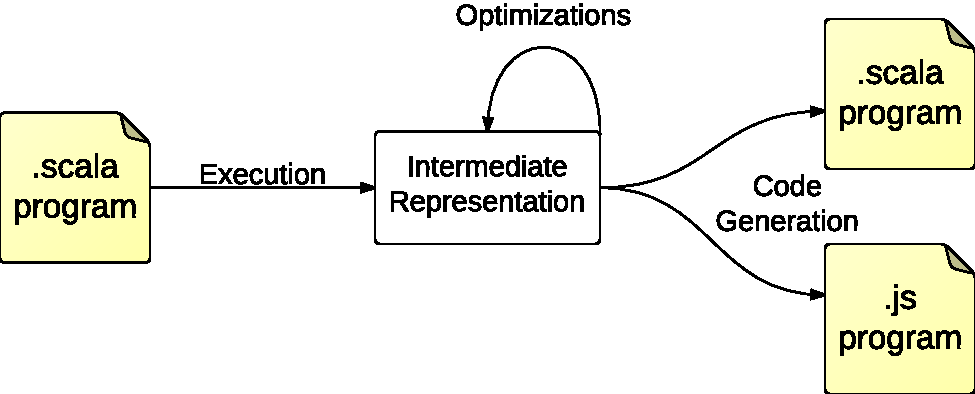
\includegraphics[width=7cm]{lms.pdf}
  \caption{Compilation of a program using LMS. An initial Scala program using embedded DSLs (on the left) evaluates
  to an intermediate representation from which the final program’s code is generated (on the right).}
  \label{lms-diagram}
\end{figure}

The bindings between stages are type-directed: a value of type \code{Rep[Int]} in the first stage will yield a value
of type \code{Int} in the second stage. If you consider the following code:
\begin{lstlisting}
val inc: Rep[Int] => Rep[Int] =
  x => x + 1
\end{lstlisting}
The function looks like
a regular Scala function excepted that its parameter type and its return type are wrapped in the \code{Rep[T]} type
constructor that denotes intermediate representations. The \code{+} operator has been defined on \code{Rep[Int]}
values and returns the intermediate representation of an addition. Finally, the \code{inc} function returns the
intermediate representation of a computation yielding the number following the value of the parameter \code{x}.

You can get a \code{T} value from a \code{Rep[T]} value by generating code from the intermediate representation and
compiling it:
\begin{lstlisting}
val compiledInc: Int => Int =
  compile(inc)
\end{lstlisting}
The \code{compile} function takes a staged program of type \code{Rep[A] => Rep[B]} and returns a final program of
type \code{A => B}.

The intermediate representation implementation is hidden for users but DSLs authors have to provide the corresponding
intermediate representation of each construct of their language. For that purpose, LMS comes with an extensible
intermediate representation implementation defining computations as a graph of statements. In the case of the
\code{inc} function, this graph contains a \code{Plus} node applied on a \code{Sym} node (the \code{x} parameter) and
a \code{Const} node (the literal value \code{1}).

Then, the code generation process consists in sorting this graph according to expressions dependencies and to emit
the code corresponding to each node. The listings \ref{codegen-js} and \ref{codegen-scala} show the JavaScript and
Scala generated code for the \code{inc} function:
\begin{multicols}{2}
\lstinputlisting[language=JavaScript, caption=JavaScript code generation, label=codegen-js]{inc.js}
\lstinputlisting[caption=Scala code generation, label=codegen-scala]{inc.scala}
\end{multicols}

Defining a DSL consists in three steps, each defining:

\begin{itemize}
\item The concrete syntax: an abstract API manipulating \code{Rep[_]} values~;
\item The intermediate representation: an implementation of the concrete syntax in terms of statement nodes~;
\item A code generator for the intermediate representation: a \emph{pretty-printer} for each DSL statement node.
\end{itemize}

\subsubsection{Example: null references}

As an illustration of the staging mechanism, we present a simple DSL to handle null references. This DSL provides an
abstraction at the stage-level that is removed by optimization during the code generation.

Null references are a known source of problems in programming languages~\cite{Hoare09_Null,Nanda09_Null}. For
example, consider the following typical JavaScript code finding a particular widget in the page and a then particular
button in the widget:

\begin{lstlisting}[language=JavaScript,label=null-unsafe,caption=Unsafe code]
var loginWidget = document.querySelector("div.login");
var loginButton = loginWidget.querySelector("button.submit");
loginButton.addEventListener("click", function (e) { ... });
\end{lstlisting}

The native \code{querySelector} method returns \code{null} if no node matched the given selector in the document. If
we run the above code in a page where the widget is not present, it will throw an error and stop further JavaScript
execution. We can write defensive code to handle \code{null} cases, but it leads to very cumbersome code:

\begin{lstlisting}[language=JavaScript,label=null-defensive,caption=Defensive programming to handle null references]
var loginWidget = document.querySelector("div.login");
if (loginWidget !== null) {
  var loginButton = loginWidget.querySelector("button.submit");
  if (loginButton !== null) {
    loginButton.addEventListener("click", function (e) { ... });
  }
}
\end{lstlisting}

Ja-scala is a DSL that has both the safety and performance of listing \ref{null-defensive} but the
expressiveness of listing \ref{null-unsafe}. We can get safety by wrapping potentially null values of type
\code{Rep[A]} in a container of type \code{Rep[Option[A]]} requiring explicit dereferencing, we can get
expressiveness by using the Scala \code{for} notation for dereferencing, and finally we can get performance by
generating code that does not actually wraps values in a container but instead checks if they are \code{null} or not
when dereferenced. The wrapping container exists only at the stage-level and is removed during the code generation.
Here is a Scala listing that uses our DSL (implementation details are given in section \ref{implementation}):

\begin{lstlisting}
for {
  loginWidget <- document.find("div.login")
  loginButton <- loginWidget.find("submit.button")
} loginButton.on(Click) { e => ... }
\end{lstlisting}

The evaluation of the above listing produces a graph of statements from which JavaScript code equivalent to
listing \ref{null-defensive} is generated.

\section{Contribution}

\subsection{DOM}

As seen in the introduction, the return type of the function creating DOM elements depends on
the value of its first parameter. Listing \ref{dom-generics} showed a statically typed interface
for the \code{createElement} function using type parameters. However, as shown in the listing,
functions taking an \code{ElementName} parameter also have to take a type parameter (\eg{} function
\code{create}). Using type parameters may lead to an explosion of use of type parameters in
the code. Instead, we propose to use path-dependent types so the dependency between the
element name and the function return type is more self-contained (no need to fill a type parameter
at use-site):

\begin{lstlisting}
class ElementName {
  type Element
}

def createElement(name: ElementName): name.Element = ...
\end{lstlisting}

We can rewrite the \code{create} function as follows:

\begin{lstlisting}
def create(name: ElementName, className: String) = {
  val el = createElement(name)
  el.className = className
  el
}
\end{lstlisting}

The \code{create} function type signature is not polluted with an extra type parameter.


\subsection{Events}

We can apply the same pattern to the \code{addEventListener} function (renamed to \code{on}):

\begin{lstlisting}
class EventName {
  type Data
}
object Click extends EventDef { type Data = MouseEvent }

def on(name: EventName)(handler: Rep[name.Data] => Rep[Unit]): Rep[Unit]

val clicks = on(Click)
clicks(event => println(event.offsetX))
\end{lstlisting}

An \code{EventName} value represents an event that carries its corresponding event data type in its
\code{Data} type member. The \code{on} method takes a parameter \code{ev} of type \code{EventDef}
and a \code{handler} parameter whose type refers to the \code{Data} member of the \code{name}
parameter, so the type of the handler depends on the \code{name} value.

The following Scala listing generates code equivalent to listing \ref{event-js} and is completely
type-safe: if the user misspells the event name or tries to use an undefined property on an event
his program won’t compile.

\begin{lstlisting}
window.on(MouseWheel) { e =>
  scale = Math.round(scale + e.wheelDeltaY / 16)
}
\end{lstlisting}

We can write a statically typed version of listing \ref{lst:react-js} as follows:

\begin{lstlisting}
val clicks = on(Click)
clicks(event => println(event))
clicks(event => alert(event))
\end{lstlisting}

\subsection{Selectors}

As presented in the introduction, the JavaScript \code{querySelector} function is polymorphic in
its return type but this return type can not \emph{always} be inferred from its parameters. A
pragmatic solution to this problem would be to return by default the most general type, to handle
cases where a more specialized return type can be safely inferred without requiring an explicit
annotation from users, and finally to handle cases where users have to down-cast the return type
while forbidding to cast to an impossible return type.

First, we start by making the return type bound to the most general return type:

\begin{lstlisting}
def find[A <: Element](selector: Rep[String]): Rep[A]
\end{lstlisting}

When calling this function, the \code{A} type parameter can be filled at use-site but can only be
filled with a type that is a subtype of \code{Element}, so we forbid cases like the following:

\begin{lstlisting}
find[Int](".title") // Does not compile
\end{lstlisting}

However, if the \code{A} type parameter is not explicitly filled by the user, the Scala compiler
infers the greatest lower bound for \code{A}: \code{Nothing}.

\begin{lstlisting}
find(".title") // Returns Rep[Nothing]...
\end{lstlisting}

We can fix that by replacing the bounded quantification by an implicit parameter \emph{witnessing}
that \code{A} can be the result of searching elements in the DOM:

\begin{lstlisting}
def find[A](selector: Rep[String])(implicit ev: Findable[A]): Rep[A]

class Findable[A]
object Findable {
  implicit val default: Findable[Element] = new Findable[Element]
  implicit def elementSub[A <: Element]: Findable[A] = new Findable[A]
}
\end{lstlisting}

If users try to fill \code{A} with \code{Int} they get a compile error (implicit not found).

So far, our definition has the most general return type by default and allows users to explicitly
ask to down-cast the result to a subtype of \code{Element}, but our definition is still unable to
automatically infer a more specialized return type when possible.

We solve this problem by making the \code{selector} parameter polymorphic too and by replacing the
previous implicit parameter by another one fixing the return type of the function according to the
selector parameter type:

\begin{lstlisting}
def find[A, B](selector: A)(implicit evidence: A Selects B): B

class Selects[A, B]
object Selects {
  // Case of selector being a String
  implicit val string: String Selects Element = new Selects[String, Element]
  implicit def elementSub[A <: Element]: String Selects A = new Selects[String, A]
  // Case of selector being an element name (cf below)
  implicit def elementName[A <: Element]: ElementName[A] Selects A =
    new Selects[ElementName[A], A]

  type ElementNameAlias[El] = ElementName { type Element = El }
  implicit def elementName: ElementNameAlias[El] Selects El
}

class ElementName[A <: Element]
val Div: ElementName[DivElement] = new ElementName[DivElement]

class ElementName {
  type Element
}
val Div: ElementName { type Element = DivElement } = new ElementName { type Element = DivElement }
\end{lstlisting}

Now users can write the following:

\begin{lstlisting}
find(".foo") // returns an Element
find[String, InputElement](".foo") // returns an InputElement
find[String, Int](".foo") // does not compile
find(Div) // returns a DivElement
find[ElementName[DivElement], Int](Div) // does not compile
\end{lstlisting}

However, now that the \code{find} function takes two type parameters, users have to supply both
if they want to explicitly down-cast the return type of the query. We can solve this problem by
creating an intermediate class:

\begin{lstlisting}
trait FindBuilder[B] {
  def apply[A](selector: A)(implicit evidence: A Selects B): B
}

def find[B]: FindBuilder[B]
\end{lstlisting}

Now users can write the following:

\begin{lstlisting}
find(".foo") // returns an Element
find[InputElement](".foo") // returns an InputElement
find[Int](".foo") // does not compile
find(Div) // returns a DivElement
find[Int](Div) // does not compile
\end{lstlisting}


\section{Evaluation}

\subsection{Events}


Other languages either provide loose information about the data type of the listened event (Dart) or
give no way to abstract over an event (GWT, Kotlin).

The most popular JavaScript library, jQuery~\cite{Bibeault08_jQuery}, used by more than 40\% of the top million
sites\footnote{\href{http://trends.builtwith.com/javascript}{http://trends.builtwith.com/javascript}} aims to
simplify RIA development. It handles the \code{null} references problem by wrapping each query result in a container
so before each further method call it tests the emptiness of the container and applies the operation effectively only
if the container is not empty. It provides an expressive API but the emptiness checking involves a slight performance
penalty since each result is wrapped and then unwrapped for the subsequent method invocation. jQuery also has an API
to turn asynchronous computations into first-class citizens. However, jQuery is just a library and thus cannot bring
type safety to JavaScript programs.

TypeScript\footnote{\href{http://www.typescriptlang.org/}{http://www.typescriptlang.org/}} is a language compiling to
JavaScript supporting classes, modules and soft typing. Because TypeScript is a superset of JavaScript, any valid
JavaScript program is a valid TypeScript program. Developers can progressively leverage TypeScript’s features to turn
their JavaScript sources into large, modular and more robust code bases. However, TypeScript does not provide advanced type feature to deal with DOM management.

The Roy~\cite{McKenna_Roy} programming language is a statically typed functional programming language compiling to
JavaScript. It features global type inference, algebraic data types, pattern matching and a sequencing notation
similar to Scala’s \code{for} notation. Roy does not address concerns such as event handling and DOM fragments
definition. It has no specific feature to deal with correctly typed FFI. 


GWT~\cite{Chaganti07_GWT} compiles Java code to JavaScript. It exposes the browser’s APIs through type-safe Java APIs
and simplifies DOM fragments definition. However, to provide correct type management, GWT provides a verbose API to deal with DOM fragment definition and event handling. New DOM Api can not be easily managed in a concise and safe way as the Java programming language does not provide advanced type feature. 

Kotlin\footnote{\href{http://kotlin.jetbrains.org/}{http://kotlin.jetbrains.org/}} is a recent language written by
JetBrains, that targets both the JVM and JavaScript. It has libraries addressing partially Web programming concerns
and supports advanced programming language features such as mixins, type inference, variance annotations for type
parameters and pattern matching. In the specific problem of the definition of concise and safe FFIs it has the same issue than GWT. 

Opa\footnote{\href{http://opalang.org/}{http://opalang.org/}} and Links~\cite{Cooper07_Links} are languages designed
for Web programming. They feature static typing with global type inference, modules and pattern matching. These
languages provide a syntactic sugar for writing HTML fragments directly in the code. The server and client parts of
an application are written in a single language and the system can decide whether a code fragment will run on
server-side, client-side or both. However, these languages are not extensible, so there is no way for developers to
customize the compilation process of their abstractions on client and server sides. Furthermore, hiding the code
execution distribution gives programmers less control on communication error handling~\cite{Guerraoui99_Distributed}.

Dart~\cite{Griffith11_Dart} is a language designed specifically for Web programming. It has been designed to have a
familiar syntax for JavaScript developers and supports soft typing, classes and a module system. It also provides a
high-level concurrent programming system similar to an actor system. Finally, Dart code can be executed on both
client and server sides but the compiler is not extensible so developers cannot customize the compilation process of
a given abstraction on client and server sides.

Table \ref{comparison} gives a synthetic view of the comparison of our work with other mainstream approaches. Lines
give features desired to write large Web applications and colums list mainstream tools for Web programming. Cells
show the support level of each feature for each tool.

TODO{Fay}

\begin{table}
\centering
\begin{tabular}{| l | c | c | c | c | c | c | c | c |}
\hline
& jQuery & TypeScript & Roy & GWT & Kotlin & Opa & Dart & js-scala \\
\hline
Type safe event handling & & & & *** & & & & *** \\
\hline
DOM definition & * & & & *** & ** & *** & * & *** \\
\hline
Static typing & & * & ** & ** & ** & ** & * & ** \\
\hline
Easiness for defining libraries & ** & *** & *** & *** & *** & *** & *** & * \\
\hline
\end{tabular}
\caption{Support of concise and safe FFI. Zero star means that the feature is not supported
at all, three stars mean a strong support.}
\label{comparison}
\end{table}

Several model-driven methodologies for creating web applications have been proposed, including
\cite{schwabe1996systematic,lima2003modeling,ceri2000web,koch2001authoring,pastor2003oows,valverde2007mda,vdovjak2003engineering,kraus2007model,nunes2006rapid,brambilla2008designing,valderas2007transformational,van2006hera,Groenewegen08_WebDSL}.
Many of them follow the standard top-down MDE vision in providing abstractions and code generators, nevertheless
these cannot be easily customized or they generate only application skeletons.



\section{Conclusion and Perspectives}


\bibliographystyle{plain}
\bibliography{biblio}

\end{document}

